\documentclass[a4,12pt]{book}
\usepackage[portuguese]{babel}
\usepackage[utf8]{inputenc}
\usepackage[portugues]{mystyle}
\usepackage{multirow}
\usepackage{multicol}
\usepackage{rotating}
\usepackage{amsmath}
\usepackage{tikz}
\usepackage{tikz-qtree}
\usepackage{clrscode}
\usepackage[hidelinks]{hyperref}
\usetikzlibrary{automata, positioning, decorations.pathmorphing}
\usepackage{biblatex}
\addbibresource[label=bib]{ref.bib}
\usepackage{listings}


\emergencystretch=2em

\DeclareFontFamily{U}{matha}{\hyphenchar\font45}
\DeclareFontShape{U}{matha}{m}{n}{
      <5> <6> <7> <8> <9> <10> gen * matha
      <10.95> matha10 <12> <14.4> <17.28> <20.74> <24.88> matha12
      }{}
\DeclareSymbolFont{matha}{U}{matha}{m}{n}
\DeclareFontSubstitution{U}{matha}{m}{n}
\DeclareMathSymbol{\abxcup}{\mathbin}{matha}{'131}

\newcounter{mycounter}
\setcounter{mycounter}{0}
\newenvironment{exercicio}{\refstepcounter{mycounter}
    {\bf Exercício~\themycounter: }
      \rmfamily}{\medskip}

\begin{document}

%\bibliographystyle{alpha}

\author{Márcio Moretto Ribeiro}

\title{Introdução à Análise de Algoritmos}

\maketitle
\tableofcontents

\include{apresentacao}
\chapter{Introdução}
\label{cha:intro}

\section{Algoritmos}

Um {\em problema computacional} é a especificação de uma relação desejada entre um certo {\em valor de entrada} escolhido em um conjunto de valores válidos e o {\em valor de saída} esperado.

\begin{example}
  {\bf Problema da busca}\\

  {\bf Entrada:} Uma sequência de $n$ valores $a_1, \dots, a_n$ em que $a_i \in \mathbb{Z}$ para $1 \leq i \leq n$ e $b \in \mathbb{Z}$.\\

  {\bf Saída:} $i \in \mathbb{N}$ tal que $a_i = b$ se existir ou $\bot$ caso contrário.


  A sequência $3, 5, 16, 17, -1$ junto do valor $5$ é uma entrada válida para este problema.
  Qualquer entrada válida é chamada de {\em instância do problema}.
  A saída esperada para essa instância é $2$, pois o valor $5$ ocorre na segunda posição da sequência.

  Outra instância do problema é dada pela mesma sequência junto do valor $42$.
  Neste caso a saída esperada é $\bot$, uma vez que o valor $42$ não ocorre na sequência.
\end{example}

\begin{example}
  {\bf Problema da 3-soma}\\

  {\bf Entrada:} Três sequência de $n \in \mathbb{N}$ valores cada $ a_1, \dots, a_n$,  $b_1, \dots, b_n$ e $c_1, \dots, c_n$ em que $a_i, b_i, c_i \in \mathbb{Z}$ para $1 \leq i \leq n$.\\

  {\bf Saída:} A quantidade de $i$s, $j$s e $k$s tais que $a_i + b_j + c_j = 0$.

  Uma instância do problema é da pelas sequências:
  \begin{itemize}
  \item[] $1, 2, 3$
  \item[] $2, 4, 6$
  \item[] $-4, -8, -10$
  \end{itemize}

  A saída esperada neste caso é $2$ porque:
  \begin{itemize}
  \item[] $2 + 2 - 4 = 0$
  \item[] $2 + 6 - 8 = 0$
  \end{itemize}
\end{example}

\begin{example}
  {\bf Problema da ordenação}\\

  {\bf Entrada:} Uma sequência de $n$ valores $a_1, \dots, a_n$ em que $a_i \in \mathbb{Z}$ para $1 \leq i \leq n$.\\

  {\bf Saída:} Uma permutação da sequência de entrada $a'_1, \dots, a'_n$ tal que $a_i \leq a_j$ para todo $i \leq j$.

  Para a instância $3, 42, 17, 2, -1$ deste problema, a saída esperada é $-1, 2, 3, 17, 42$.
\end{example}


A disciplina de Introdução à Teoria da Computação (ITC) tem como objeto de estudo os problemas computacionais.
Como eles se classificam entre os que tem solução ou não e entre os que tem solução eficiente ou não.
A solução de um problema computacional é um algoritmo.

Os objetos de estudo desta disciplina são os algoritmos.
Mas afinal, o que são algoritmos?

Um {\em algoritmo} parte de uma entrada escolhida em um conjunto potencialmente infinito de possibilidades ({\em princípio da massividade}) para produzir um valor de saída.
O algoritmo processa a entrada por meio de uma sequência de passos ({\em princípio da discretude}) que produzem valores intermediários.
Cada passo  segue uma instrução simples ({\em princípio da elementaridade}) que só depende dos valores anteriores, não admitindo ambiguidades ({\em princípio da exatidão}) \cite{malcev70}.

Um {\em prorgrama} é a realização de um algoritmo em certa {\em linguagem de programação}.
Assim, um algoritmo é, de um lado, a solução de um problema de computação e, de outro, uma abstração de um conjunto de programas, ele é a idéia por trás desses programas.

Um algoritmo é {\em correto} se para toda instância do problema ele produz a saída esperada depois de uma sequência finita de passos.
Nesse caso dizemos que o algoritmo {\em resolve} o problema.

Há uma controversa se devemos ou não considerar uma sequência infinita de instruções como um algoritmo.
Essa questão, complicada, está no coração do nascimento da ciência da computação e será tratada em ITC.
Neste curso focaremos nos algoritmos corretos e, assim, escaparemos dela.

Para enfatizar o fato de que algoritmos abstrações de programas, eles serão apresentados neste curso em uma linguagem informal conhecida como {\em pseudo-código}.

\begin{example}
  Considere a seguinte solução para o problema da busca.

\begin{codebox}
\Procname{$\proc{BuscaSequencial}(A, b)$}
\li \Comment Recebe $a_1, \dots, a_n$ com $a_i \in \mathbb{Z}$ e $b \in \mathbb{Z}$
\li \Comment Devolve $i$ tal que $a_i = b$ se existir e $\bot$ caso contrário
\li \For $i \gets 1$ até $n$
\li \Do \If $a_i = b$
\li     \Then \Return $i$
        \End
    \End
\li \Return $\bot$
\End
\end{codebox}


As duas primeiras linhas são apenas comentários que explicitam a especificação do problema que o algoritmo resolve.
A linha 3 indica que um certo valor $i$ deve variar de $1$ até $n$.
As duas linhas seguintes estabelecem que se $a_i$ for igual a $b$ então o valor de $i$ deve ser devolvido como resposta do problema.
Por fim, a última linha indica que se o algoritmo chegou naquele ponto, então o valor $\bot$ deve ser devolvido como solução do problema.

\end{example}

Esta disciplina estuda algoritmos.
Como podemos garantir que certo algoritmo resolve um problema, ou seja, que ele é correto?
O algoritmo do exemplo acima está correto?
Por que?
Como podemos comparar duas soluções distintas para um mesmo problema?
Ou seja, se conhecemos dois um mais algoritmos corretos para um mesmo problema, como avaliamos qual é melhor?
O algoritmo do exemplo acima é o melhor algoritmo possível para o problema da busca?
Como podemos garantir isso?

Avaliaremos os algoritmos corretos a partir da quantidade de recursos que eles consomem.
Estudaremos particularmente dois recursos: espaço de memória e, principalmente, o tempo de execução.

Nos capítulos seguintes veremos uma série de algoritmos para resolver alguns problemas centrais da computação como o problema da busca e da ordenação.
Em cada caso avaliaremos os algoritmos apresentados quanto sua corretude e sua eficiência em consumo de tempo e espaço de memória.

No Capítulo X apresentaremos o estudo dos algoritmos a partir do método empírico.
Relembraremos o método e veremos um exemplo comparando o tempo de execução de duas soluções para o problema da busca em sequências ordenadas.
Então exploraremos técnicas para arrsicar modelos matemáticos adequados para avaliar o consumo de tempo dos algoritmos.
E finalmente veremos ferramentas matemáticas uteis para comparar funções quanto ao seu crescimento, a chamada notação assintótica.
No Capitulo X estudaremos algoritmos de ordenação como estudo de caso da teoria apresentada anteriormente.
Veremos uma série de algoritmos que resolvem o mesmo problema e utilizaremos as técnicas apresentadas para construir e testar modelos do consumo de tempo deles.
Estudaremos também um limite teórico da eficiência do problema da ordenação e veremos dois algoritmos que superam esse limite utilizando mais informações do que as assumidas no enunciado do teorema.
Concluiremos a apostila no Capítulo X apresentando algoritmos e técnicas um pouco mais avançãdos como programação dinâmica e análise amortizada.


\chapter{Método Empírico}

Esquematicamente, o método empírico pode ser descrito por cinco fases:
\begin{enumerate}
\item {\em Observação:} medições sobre algum aspecto do mundo
\item {\em Hipótese:} concepção de um modelo consistente com as observações
\item {\em Predição:} eventos são previstos de acordo com o modelo
\item {\em Verificação:} as predições são testadas fazendo-se novas observações
\item {\em Validação:} o processo se repete ajustando o modelo até que ele concorde com as observações
\end{enumerate}

Dois pontos centrais sobre o método empírico é que as verificações devem ser {\em reprodutíveis} e as hipóteses {\em falseáveis}.
Uma hipóstese que não pode ser falseada por observações (empíricamente) não é científica e a o processo de verificação deve poder ser feito por outros cientístas independentes.

O aspecto do mundo que pretendemos investigar nesta disciplina é o tmepo de processamento de um algoritmo.
Lembre-se, porém, que um algoritmo é uma ideia que precede o advento dos computadores.
O algoritmo de Euclídes, por exemplo, data de 300 a.C., ou seja, séculos antes dos primeiros computadores começarem a ser construídos nos anos 40.
Embora o algoritmo seja um conceito matemático, uma série de pesquisadores tiveram a ideia de investigá-los de maneira empírica no final dos anos 60.
A série de livros The Art of Programing, de Donald Knuth, é um marco dessa abordagem dos estudos de algoritmos \cite{knuth97}.

Em nosso recorte, observaremos o tempo de processamento da execução de um programa para diferentes entradas.
Considere, por exemplo, o algoritmo para o problema da Busca apresentado no capítulo anterior:

\begin{codebox}
\Procname{$\proc{BuscaSequencial}(A, b)$}
\li \For $i \gets 1$ até $n$
\li \Do \If $a_i = b$
\li     \Then \Return $i$
        \End
    \End
\li \Return $\bot$
\End
\end{codebox}

Vamos implementar esse algoritmo na linguagem C de maneira direita:

\begin{lstlisting}[language=C]
  // devolve a posicao de n no arranjo ou -1 se nao encontrar
  int buscasequencial(int* array, int n, int size){
    int i;
    for(i = 0; i < size; i++)
      if(array[i] == n)
        return i;
    return -1;
  }      
\end{lstlisting}

Realizamos observações usando uma máquina específica (um notebook Dell com processador intel core i7 de $8^a$ geração de 1,9GHz) em um sistema operacional específico (Linux 5.11).
Medimos o tempo total de 300 buscas mal sucedidas em arranjos de tamanhos diferentes com valores inteiros positivos calculados aleatoriamente\footnote{Mais precisamente os valores seguem uma sequência pseudo-aleatória partindo de uma semente incial.}.
Os programas que calcula o tempo da busca e que gera as entradas estão disponíveis em \url{https://github.com/marciomr/IAA}.
Variamos o tamanho do arranjo entre um milhão e dez milhões.
Obtivemos o seguinte resultado para dez observações:

\begin{table}
  \label{tab:observacao}
  \begin{tabular}{|c|c|}
    \hline
    tamanho do arranjo em milhões & tempo de 300 buscas em segundos \\
    \hline 
    1                             & 0,99                            \\
    2                             & 2,08                            \\
    3                             & 3,12                            \\
    4                             & 3,99                            \\
    5                             & 5,05                            \\
    6                             & 5,94                            \\
    7                             & 7,03                            \\
    8                             & 7,92                            \\
    9                             & 8,93                            \\
    10                            & 9,85                            \\
    \hline
  \end{tabular}
\end{table}

As observações sugerem que para cada um milhão de valores no arranjo, o tempo de processamento aumenta mais ou menos um segundo.
Essa poderia ser nossa hipótese, mas podemos fazer algo um pouco mais sofisticado.
Vamos plotar os valores da tabela em um gráfico (Figura \ref{fig:observacao}).

\begin{figure}[htp]
  \label{fig:observacao}
  \includegraphics[width=0.9\textwidth]{imagens/grafico1.png}
  \caption{Tempo de processamento da busca sequencial.}
\end{figure}

Como os pontos estão mais ou menos alinhados e como é razoável supor que um arranjo sem nenhum elemento retornaria instantaneamente o resultado, faremos a hipótese de que o tempo de processamento segue uma função linear partindo do zero.
Ou seja, a seguinte função descreve o tempo de processamento da nossa implementação em nosso ambiente:

\begin{displaymath}
t(x) = a.x
\end{displaymath}

Podemos então usar uma regressão linear para estimar o valor de $a$ que minimize a distância desse reta para cada um dos pontos.
Obtemos então o valor $a = 0,997$.
Na Figura \ref{fig:hipotese} plotamos a função $t(x) = 0,997x$ no gráfico anterior.

\begin{figure}[htp]
  \label{fig:hipotese}
  \includegraphics[width=0.9\textwidth]{imagens/grafico2.png}
  \caption{Gráfico ilustrando a hipótese de que o tempo de processamento da busca sequencial segue a função linear $t(x) = 0,997x$.}
\end{figure}

Podemos agora testar nossa hipótese de que o tempo de processamento da nossa implementação da busca sequencial para outros valores ainda não observados.
A segunda coluna da Tabela \ref{tab:verificacao} mostra os valores previstos pela hipótese para o tempo de processamento para entradas de tamanho 11 a 15 milhões.
Finalmente, podemos testar a hipótese.
Na última coluna da mesma tabela indicamos os valores observados para essas entradas:

\begin{table}
  \label{tab:verificacao}
  \begin{tabular}{|c|c|c|}
    \hline
    tamanho do arranjo em milhões & tempo previsto & tempo observado \\
    \hline 
    11                             & 10,97         & 10,87           \\
    12                             & 11,97         & 11,81           \\
    13                             & 12,97         & 12,78           \\
    14                             & 13,96         & 14,00           \\
    15                             & 14,96         & 14,74           \\
    \hline
  \end{tabular}
  \caption{Tempo de processamento previsto e observado para tamanhos maiores de arranjos.}
\end{table}

Os valores observados são notavelmente próximos aos previstos.
Ou seja, nossa hipótese foi verificada.
Poderíamos neste momento utilizar um teste estatístico para verificar nossa hipótese, mas isso foge do escopo desta disciplina.
Por hora diremos apenas que os dados parecem verificar a hipótese.

Consideremos agora a seguinte versão modificada do Problema da busca:

\vspace{0.5cm}

{\bf Problema da busca em uma sequência ordenada}\\

{\bf Entrada:} Uma sequência de $n$ valores $a_1, \dots, a_n$ em ordem crescente, isto é, $a_i \leq a_j$ para todo $i \leq j$ e $b \in \mathbb{Z}$.\\

{\bf Saída:} $i \in \mathbb{N}$ tal que $a_i = b$ se existir ou $\bot$ caso contrário.

\vspace{0.5cm}

Note que este problema é uma versão restrita do problema anterior.
Assim, toda solução do Problema da busca é também uma solução para o Problema da busca em uma sequência ordenada -- o inverso não é necessariamente verdadeiro.
Em particular, o algoritmo de Busca Sequêncial resolve ambos os problemas.
O seguinte algoritmo, por sua vez, resolve apenas o segundo:

\begin{codebox}
  \Procname{$\proc{BuscaBinaria}(A, b)$}
  \li \Comment Recebe uma sequência ordenada $a_1, \dots a_n$ e um valor $b$ todos inteiros
  \li \Comment Devolve $i$ tal que $a_i = b$ ou $\bot$ caso $b$ não ocorra na sequência
  \li $i \gets 1$
  \li $j \gets |A|$
  \li \While $i \leq j$
  \li \Do $m \gets \left \lfloor{\frac{j+i}{2}}\right\rfloor$
  \li \If $b < a_m$
  \li     \Then $j \gets m - 1$
  \li \Else
      \If $b > a_m$
  \li      \Then $i \gets m + 1$
  \li \Else \Return m 
      \End
  \End
  \End
  \li \Return $\bot$
\end{codebox}

Este algoritmo é um pouco mais sofisticado do que o anterior.
Começamos avaliando o elemento no centro da sequência ($a_m$).
Como a sequência está em ordem crescent, se o valor procurado ($b$) for maior do que $a_m$ então ele deve estar depois do valor central e podemos ignorar todos os valores anteriores a $m$.
Analogamente, se $b$ for menor que $a_m$ ele deve estar antes de $m$ e podemos ignorar todos os valores posteriores.

Como fizemos no exemplo anterior, vamos avaliar o tempo de processamento deste algoritmo utilizando o método empírico.
O primeiro passo é fazer algumas observações.
Vamos repetir as observações feitas no exemplo anterior.

\begin{table}
  \label{tab:observacao2}
  \begin{tabular}{|c|c|}
    \hline
    tamanho do arranjo em milhões & tempo de 300 buscas em segundos \\
    \hline 
    1                             & 0,00                            \\
    2                             & 0,00                            \\
    3                             & 0,00                            \\
    4                             & 0,00                            \\
    5                             & 0,00                            \\
    6                             & 0,00                            \\
    7                             & 0,00                            \\
    8                             & 0,00                            \\
    9                             & 0,00                            \\
    10                            & 0,00                            \\
    \hline
  \end{tabular}
\end{table}

As observações sugerem que o novo algoritmo é muito mais eficiente do que o primeiro.
Porém, elas não nos ajudam a conceber um modelo.

Façamos então observações com mais repetições.
Depois de alguns testes aprendemos que repetindo dez milhões de buscas o tempo de processamento passa a ser mensurável.

\begin{table}
  \label{tab:observacao3}
  \begin{tabular}{|c|c|}
    \hline
    tamanho do arranjo em milhões & tempo de 10M buscas em segundos \\
    \hline 
    1                             & 0,66                            \\
    2                             & 0,64                            \\
    3                             & 0,60                            \\
    4                             & 0,59                            \\
    5                             & 0,62                            \\
    6                             & 0,63                            \\
    7                             & 0,63                            \\
    8                             & 0,63                            \\
    9                             & 0,66                            \\
    10                            & 0,65                            \\
    \hline
  \end{tabular}
\end{table}

Desta vez conseguimos fazer as medições.
As observações sugerem que o tempo de processamento é independente do tamanho do arranjo.
Para arranjos de qualquer tamanho o tempo de procesamento parece ser maior ou menos o mesmo.
Podemos então levantar a hipótese de que o tempo de processamento é constante:

\begin{displaymath}
  t(x) = a
\end{displaymath}

Para calcular o valor de $a$ peguemos a média das observações $a = 0,63$.

\begin{figure}[htp]
  \label{fig:hipotese2}
  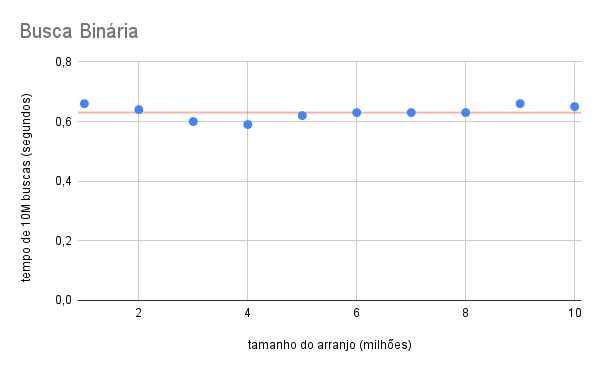
\includegraphics[width=0.9\textwidth]{imagens/grafico3.png}
  \caption{Gráfico ilustrando a hipótese de que o tempo de processamento da busca binária segue a função constante $t(x) = 0,63$.}
\end{figure}

Assim, nosso modelo preveria que para entradas de qualquer tamanho, o tempo de processamento seria próximo a $0,63$ segundos.
Vamos testar essa hipótese com entradas de tamanhos bem maior para ver se a hipótese se verifica.

\begin{table}
  \label{tab:verificacao}
  \begin{tabular}{|c|c|c|}
    \hline
    tamanho do arranjo em milhões & tempo previsto & tempo observado \\
    \hline 
    20                            & 0,63           & 0,68            \\
    100                           & 0,63           & 0,75            \\
    500                           & 0,63           & 0,81            \\
    1000                          & 0,63           & 0,89            \\
    \hline
  \end{tabular}
  \caption{Tempo de processamento previsto e observado para tamanhos maiores de arranjos.}
\end{table}

O processamento continua muito rápido mesmo para arranjos bem grandes, mas parece que a hipótese não foi verificada.
Seguindo o método empírico, devemos fazer novas observações para tentar formular uma nova hipótese.
Tentemos repetir nossas observações com uma maior amplitude de valores.
Ao invés de aumentar o tamanho de nossa sequência em um tamanho fixo a cada observação, vamos tentar desta vez dobrar o tamanho da sequência a cada observação.


\begin{table}
  \label{tab:observacao4}
  \begin{tabular}{|c|c|}
    \hline
    tamanho do arranjo em milhões & tempo de 10M buscas em segundos \\
    \hline 
    1                             & 0,59                            \\
    2                             & 0,62                            \\
    4                             & 0,69                            \\
    8                             & 0,69                            \\
    16                            & 0,74                            \\
    32                            & 0,76                            \\
    64                            & 0,79                            \\
    128                           & 0,83                            \\
    256                           & 0,96                            \\
    512                           & 1,01                            \\
    \hline
  \end{tabular}
\end{table}

As observações sugerem que o tempo de processamento cresce linearmente conforme dobramos o tamanho da nossa entrada.
Podemos arriscar então que o tempo de processamento segue o seguinte modelo:

\begin{displaymath}
  t(2^y) = a.y + b
\end{displaymath}

\begin{figure}[htp]
  \label{fig:hipotese3}
  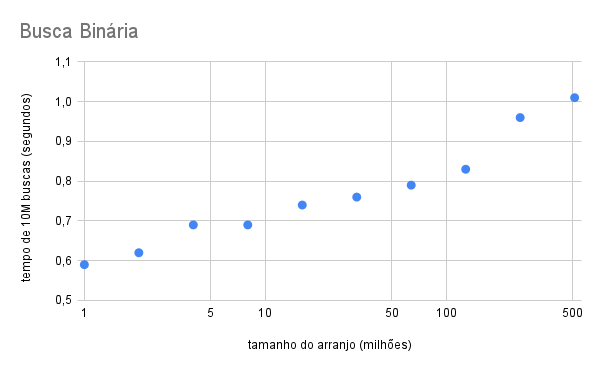
\includegraphics[width=0.9\textwidth]{imagens/grafico4.png}
  \caption{Gráfico ilustrando a hipótese de que o tempo de processamento da busca binária segue a função constante $t(2^y) = a.y + b$.}
\end{figure}

Como fizemos no exemplo anterior, podemos computar os valores de $a$ e $b$ utilizando uma técnica de regressão linear.
Ficamos assim com $a = 0,043$ e $b = 0,529$.

Por fim, mudamos a variável $2^y = x$ e obtemos a seguinte equação:

\begin{displaymath}
  t(x) = a.log_2(x) + b = 0,043.log_2(x) + 0,529
\end{displaymath}


\chapter{Correção}

No capítulo anterior vimos que é possível utilizar o método empírico para avaliar tempo de processamento de diferentes soluções para um mesmo problema.
Neste capítulo daremos um passo atrás.
Como podemos garantir, para começo de conversa, que um algoritmo de fato resolve um problema?
Em outras palavras, como podemos provar a correção de um algoritmo?

Para provar a correção de um algoritmo iremos usar uma forma de prova por indução.
Assim, antes de partir para os exemplos de prova por indução em um algoritmo, vale a pena relembrar como funciona uma prova por indução em um contexto mais típico.

Normalmente, uma prova por indução é usada para provar alguma propriedade sobre números naturais.
A ideia de uma prova por indução é relativamente simples.
Ela se divide em três etapas.
Primeiro precisamos provar que a propriedade vale para o $0$ ou para o primeiro número que nos interessa.
Isso é chamado de {\em Base da Indução}.
Então supomos que a propriedade vale para um número $n$, {\em Hipótese da Indução}.
Por fim, provamos que se vale para $n$ então vale para $n+1$, {\em Passo de Indução}.
Assim, mostramos que vale para $0$ e se vale para $0$, deve valer para $1$, e se vale para $1$, deve valer para $2$ e assim por diante.
Com isso, provamos que a propriedade vale para todos os números naturais.

Vejamos um exemplo.
Considere a seguinte somatória:

\begin{displaymath}
  1 + 2 + 3 + \dots + n = \sum_{i=1}^n i = \frac{n(n+1)}{2}
\end{displaymath}

Vamos provar por indução que esse resultado vale para qualquer número natural $n$.

O primeiro passo é provar a base da indução.
Vamos provar que o resultado vale para $n = 1$

\begin{displaymath}
  1 = \frac{1(1+1)}{2}
\end{displaymath}

Agora vamos explicitar a Hipótese de Induação.

\begin{displaymath}
  1 + 2 + 3 + \dots + n = \frac{n(n+1)}{2}
\end{displaymath}

Por fim, fazemos o Passo de Indução.

\begin{eqnarray*}
  1 + 2 + 3 + \dots + n + n + 1 & = & \frac{n(n+1)}{2} + n + 1 \\
  & = & \frac{n^2 + n + 2n + 2}{2} \\
  & = & \frac{n^2 + 3n + 2}{2} \\
  & = & \frac{(n+1)(n+2)}{2} \\
\end{eqnarray*}

Note que a primeira equação vale por conta da Hipótese de Indução.

Passemos agora para um problema computacional.
Continuemos considerando o problema da busca em uma sequência ordenada e os dois algoritmos que conhecemos para ele.
Primeiro o algoritmo da busca sequencial:

\begin{codebox}
\Procname{$\proc{BuscaSequencial}(A, b)$}
\li \For $i \gets 1$ até $n$
\li \Do \If $a_i = b$
\li     \Then \Return $i$
        \End
    \End
\li \Return $\bot$
\End
\end{codebox}

Para mostrar que o algoritmo é correto temos que incontrar um {\em invariante}.
Uma propriedade que vale em todas as iterações.
No nosso caso, vamos considerar a linha 2 do algoritmo e a propriedade será a seguinte:

\begin{displaymath}
b \textrm{ não ocorre em } a_1, \dots, a_{i-1}
\end{displaymath}

Vamos provar que essa propriedade é de fato invariante usando a técnica da indução.

Primeiro temos que provar que ela vale para $i = 1$.
Essa é a base da indução.

Para isso basta notar que neste caso a sequência é vazia e, portanto, $b$ não pertence a ela.

A Hipótese de Indução já foi explicitada.
Para mostrar o passo de indução vamos supor a HI e mostrar que a propriedade continua valendo para $i+1$.
Se $b$ estivesse na sequência $a_1 \dots a_i$ então, pela HI, $b = a_i$.
Neste caso, não chegaríamos na linha 2, porque o algoritmo teria encerrado antes disso.

Assim, sempre que chegamos na linha 2, $b$ não ocorre em $a_1, dots, a_{i-1}$.
Portanto, quando chegamos na 3, é a primeira vez em que $a_i = b$.
E se chegarmos na linha 4, sabemos que $b$ não ocorre em $a_1, \dots, a_n$.


Vamos agora para nosso segundo exemplo:


\begin{codebox}
  \Procname{$\proc{BuscaBinaria}(A, b)$}
  \li $i \gets 1$
  \li $j \gets |A|$
  \li \While $i \leq j$
  \li \Do $m \gets \left \lfloor{\frac{j+i}{2}}\right\rfloor$
  \li \If $b < a_m$
  \li     \Then $j \gets m - 1$
  \li \Else
      \If $b > a_m$
  \li      \Then $i \gets m + 1$
  \li \Else \Return m 
      \End
  \End
  \End
  \li \Return $\bot$
\end{codebox}

Vamos mostrar que as seguintes propriedades são invariantes na linha 4:

\begin{displaymath}
b \textrm{ não ocorre em } a_1, \dots, a_{i-1}
\end{displaymath}

\begin{displaymath}
b \textrm{ não ocorre em } a_{j+1}, \dots, a_n
\end{displaymath}

A base da indução é simples, no primeiro momento $i = 1$ e $j = n$.
Portanto ambas propriedades valem porque as duas sequências são vazias nessas condições.

Vamos supor que a propriedade vale em um certo momento quando chegamos na linha 4.
Agora imagine que chegamos mais uma vez nessa linha.
Neste caso, não saímos do laço.
Portanto, uma de duas coisas teve que ocorrer:
$b < a_m$ ou $b >a_m$.

No primeiro caso, temos que $j = m-1$.
Como a sequência está ordenada, $b$ não ocorre em $a_{j+1} = a_m, \dots, a_n$ porque $b < a_m$.
Além disso, pela hipótese de indução, temos que $b$ não ocorre em $a_1, \dots, a_{i-1}$.

No segundo caso, temos que $i = m+1$.
Como a sequência está ordenada, $b$ não ocorre em $a_{1} = a_{1}, \dots, a_n$ porque $b > a_m$.
Além disso, pela hipótese de indução, temos que $b$ não ocorre em $a_{j+1}, \dots, a_n$.

O invariante vale sempre na linha 4.
Se chegarmos na linha 9 é proque $a_m = b$ e se chegarmos na linha 10 é porque $b$ não está nem em $a_1, \dots, a_i$ nem em $a_j, \dots, a_n$ e $i > j$.
Portanto $b$ não está em $a_1, \dots, a_n$.

\vspace{2cm}

\begin{exercicio}
  Considere o seguinte algoritmo:

\begin{codebox}
  \Procname{$\proc{3Soma}(A, B, C)$}
  \li $n \gets 0$
  \li \For $i \gets 1$ até $n$
  \li \Do \For $j \gets 1$ até $n$
  \li     \Do \For $k \gets 1$ até $n$
  \li         \If $a_i + b_j + c_k = 0$
  \li         \Then $n \gets n + 1$
  \End
  \End
  \End
  \li \Return $n$
\end{codebox}

Prove que este algoritmo resolve o problema da 3-soma apresentado no Capítulo \ref{cha:intro}.
  
\end{exercicio}

\chapter{Modelos}

Vimos no Capítulo \ref{} que podemos avaliar o tempo de processamento de um algoritmo usando o método empírico.
Para isso, em algum momento precisamos de um {\em modelo} que iremos testar.
Nos exemplos que vimos o modelo foi tirado intuitivamente a partir das observações.
Há métodos mais adequados para conceber um modelo para o consumo de tempo de um algoritmo.

Vamos mais uma vez considerar os algortimos de busca que temos estudado.

\begin{codebox}
\Procname{$\proc{BuscaSequencial}(A, b)$}
\li \For $i \gets 1$ até $n$
\li \Do \If $a_i = b$
\li     \Then \Return $i$
        \End
    \End
\li \Return $\bot$
\End
\end{codebox}

Quando esse algoritmo for implementado e executado em uma máquina, as instruções seguidas tomarão um tempo que depende de uma série de fatores.
A atualização da variável $i$ na linha 1, por exemplo, deve tomar um tempo.
Digamos que esse tempo seja representao por $c_1$.
A comparação de $a_i$ com $b$ na linha 2 deve tomar algum tempo, digamos $c_2$.
Devolver um valor na linha 3 tomará tempo $c_3$ e devolver o erro na linha 4 tomará tempo $c_4$.

Não sabemos exatamente quanto é esse tempo e ele deve variar dependendo da máquina, do sistema operacional e outros fatores.
A suposição que faremos é apenas que o tempo é constante.
Deve variar ligeiramente o tempo que uma máquina leva para atualizar a variável $i$, mas essa variação deve ficar em torno de uma média.
Portanto, é razoável supor que esse tempo é constante.

O que devemos fazer, então é contar o número de vezes que cada operações ocorre.
A primeira e a segunda linha ocorrerão no máximo $n$ vezes.
Já a terceira e a quarta linha no máximo uma vez.
Assim, um bom modelo para o cosumo de tempo que este algoritmo deve tomar em função do tamanho da sequência $n$ é:

\begin{displaymath}
  t(n) \leq c_1.n + c_2.n + c_3 + c_4 
\end{displaymath}

Nosso modelo varia com o tamanho e com os valores da entrada.
Se quisermos um modelo que varia apenas com o tamanho, precisamos fazer alguma suposição.
Na maior parte deste curso faremos uma {\em análise de pior caso}.
No nosso exmeplo, o pior caso ocorre quando o elemento $b$ não está na sequência $A$.

Em algumas situações específicas é útil fazer uma análise de caso médio.
Mas em geral não conhecemos o suficiente sobre a distribuição de probabilidade da entrada.
Uma análise de pior caso nos dá um limite de quanto tempo o processamento dos dados tomará levando em conta apenas o tamanho da entrada.

No nosso caso, o modelo ficaria assim:

\begin{displaymath}
  t(n) = c_1.n + c_2.n + c_3 + c_4 = (c_1 + c_2).n + c_3 + c_4 = a.n + b
\end{displaymath}

Note que chegamos no mesmo modelo que apresentamos no Capítulo \ref{}.

Vamos agora replicar esse mesmo tipo de análise para nosso outro algoritmo.
\begin{codebox}
  \Procname{$\proc{BuscaBinaria}(A, b)$}
  \li $i \gets 1$
  \li $j \gets |A|$
  \li \While $i \leq j$
  \li \Do $m \gets \left \lfloor{\frac{j+i}{2}}\right\rfloor$
  \li \If $b < a_m$
  \li     \Then $j \gets m - 1$
  \li \Else
      \If $b > a_m$
  \li      \Then $i \gets m + 1$
  \li \Else \Return m 
      \End
  \End
  \End
  \li \Return $\bot$
\end{codebox}

Vamos atribuir constantes $c_1, dots, c_{10}$ para o tempo de processamento de cada uma das 10 linhas do algoritmo.
Agora vamos contar as linhas.
As linhas 1, 2 serão executadas uma vez cada.
Contar as demais linhas é mais complicado.

Primeiro vamos lembrar que faremos uma análise de pior caso.
Assim, a linha 9 não será executada nunca e a 10 será executada apenas uma vez.
Outra observação é que toda vez que executarmos a linha 4, executaremos ou as linhas 5 e 6 ou as linhas 7 e 8.
Para simplificar, vamos supor que o tempo de execução da linha 5 é o mesmo que da 7 ($c_5$) e que o tempo de execução da linha 6 é o mesmo que da 8 ($c_6$).
Digamos que entremos $x$ vezes no laço.
Então nosso modelo até aqui é:

\begin{displaymath}
  t(n) = c_3.x + c_4.x + c_5.x + c_6.x + c_1 + c_2 + c_{10} = (c_3 + c_4 + c_5).x + c_1 + c_2 + c_{10} = a.x + b 
\end{displaymath}

Precisamos agora calular $x$ em termos de $n$.

Para simplificar ainda mais um pouco nosso trabalho, vamos supor que o tamanho da sequência $n$ é uma potência de 2, ou seja, $n = 2^y$ para algum $y$.
Agora note que cada vez que entramos no laço, metade da sequência é descartada.

Na primeira iteração o pedaço da sequência que estamos considerando é $n = 2^y$.
Na segunda iteração ele tem tamanho $\frac{n}{2} = 2^{y-1}$.
Na terceira ele tem tamanho $\frac{n}{4} = 2^{y-2}$
Esse processo ira continuar até que o tamanho da nossa sequência seja $1 = 2^0$.
Ou seja, do começo ao final do processo as linhas 3 - 6 serão executadas $y$ vezes.
Como $n = 2^y$ temos que $y = log_2(n)$.

Neste curso, o logaritmo na base 2 será tão comum que vale a pena usar uma abreviação para ele.
Escreveremos apenas $lg$.

Assim, nosso modelo fica:
\begin{displaymath}
  t(n) = a.lg(n) + b 
\end{displaymath}

Mais uma vez, o modelo que chegamos ao contar o número de repetições de cada linha coincide com o modelo que chegamos a partir das observações.



\chapter{Crescimento de Funções}

Os modelos que aprendemos a construir para avaliar o tempo de processamento de um algoritmo contém uma série de constantes que dependem do contexto em que os experimentos serão feitos -- processador, memória, sistema operacional etc.
Uma teoria para comparar algoritmos deveria abstrair esses valores e focar apenas naquilo que se mantém válido em todos os contextos.

Assim, quando comparamos a eficiência de dois algoritmos vamos comparar o tempo processamento de cada um deles como uma função do tamanho da entrada.
Além disso, vamos focar especificamente no que acontece para valores grandes da entrada.
Em outras palavras, vamoas analisar as funções de maneira {\em assintótica}.

Considere os dois modelos que vimos no capítulo anterior:

\begin{eqnarray*}
  g(n) & = & a \cdot n + b\\
  f(n) & = & c \cdot log_2(n) + d
\end{eqnarray*}

Dependendo das constantes $a$, $b$, $c$ e $d$, os valores de $f(n)$ podem ser maiores do que de $g(n)$ para certos valores de $n$.
Mas o $g$ cresce tão mais rápido que $f$ que conforme aumentamos o valor de $n$, eventualmente $g$ supera $f$ e se mantém maior para sempre independente dos valores das constantes.
Dizemos que, assintoticamente $g$ cresce mais rápido do que $f$.

De fato, nos experimentos que fizemos, é possível notar que a busca binária é mais eficiente do que a sequencial apenas quando começamos a testar com sequências grandes.

\begin{figure}
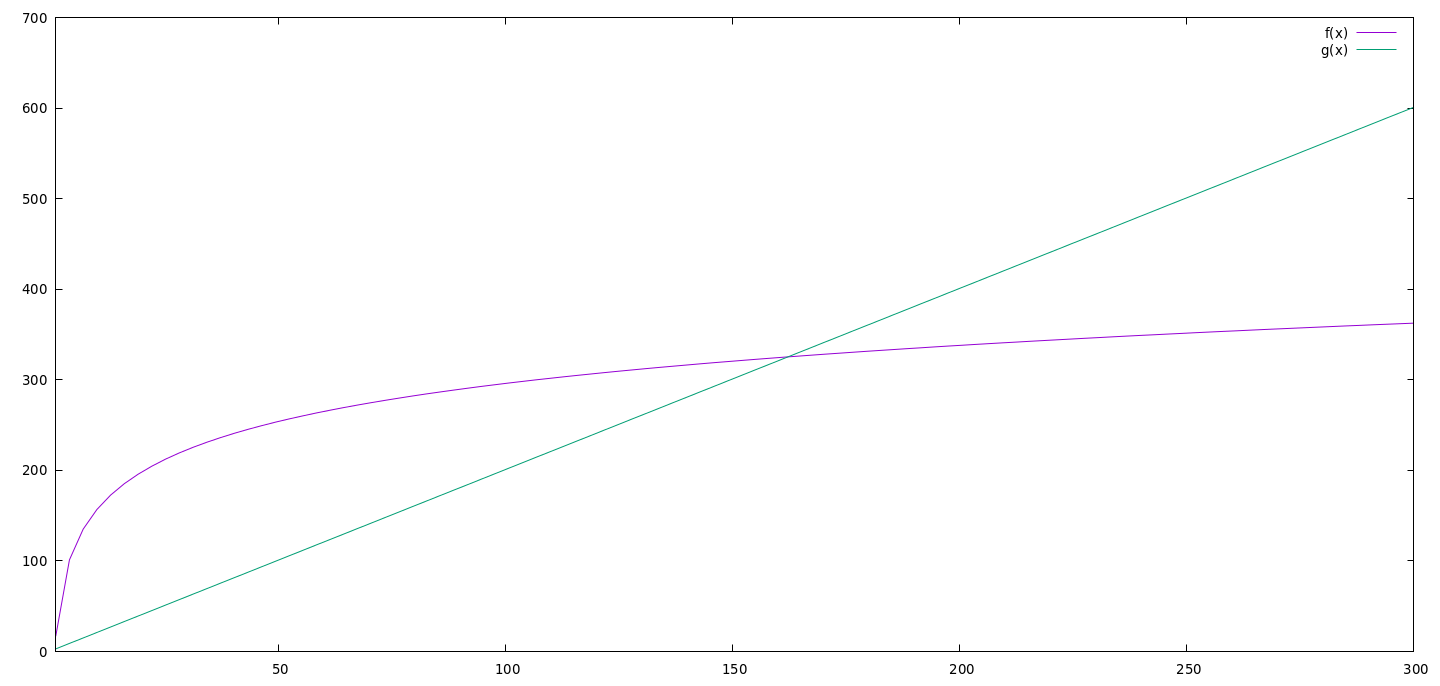
\includegraphics[width=\textwidth]{imagens/grafico7.png}
\caption{Crescimento das funções $g(n) = 2n+1$ e $f(x) = 42 \cdot log_2(n) + 17$. Há um ponto em que as curvas se cruzam e então $g(n)$ passa a ser sempre maior do que $f(n)$.}
\end{figure}

Como nos interessa analisar o comportamento assintótico das funções, trataremos como equivalentes funções que crescem de maneira similar uma vez que abstraimos as constantes.

A notação $\Theta$ formaliza matematicamente essa ideia:

\begin{displaymath}
  \Theta(g(n)) := \{ f(n) : \exists c_1, c_2, n_0 \textrm{ tal que } 0 \leq c_1 g(n) \leq f(n) \leq c_2 g(n) \forall n \geq n_0 \}
\end{displaymath}

Ou seja, $\Theta(g(n))$ é o conjunto de todas as funções que crescem de maneira parecida com $g$, que são {\em assintoticamente equivalentes} a $g$.

\begin{example}
  \begin{displaymath}
    3  n^2 + 2 n \in \Theta(n^2) 
  \end{displaymath}

  Para mostrar isso, temos que encontrar constantes $c_1$, $c_2$ e $n_0$ tais que $0 \leq c_1 n^2 \leq 3 n^2 + 2 n \leq c_2 n^2$ para todo $n \geq n_0$.

  Vamos considerar apenas valores de $n \geq 1$.
  Neste caso, $n^2$ é sempre positivo e podemos dividir tudo por $n^2$ sem alterar a direção das ineqações.
  Obtemos então:

  \begin{displaymath}
   c_1 \leq 3 + \frac{2}{n} \leq c_2
  \end{displaymath}

  Agora fica fácil ver que para $c_1 = 3$ e $c_2 = 5$ temos que as inequações valem para qualquer $n \geq 1$:

  \begin{displaymath}
   3 n^2 \leq 3 n^2 + 2n \leq 5 n^2
  \end{displaymath}

  \begin{figure}
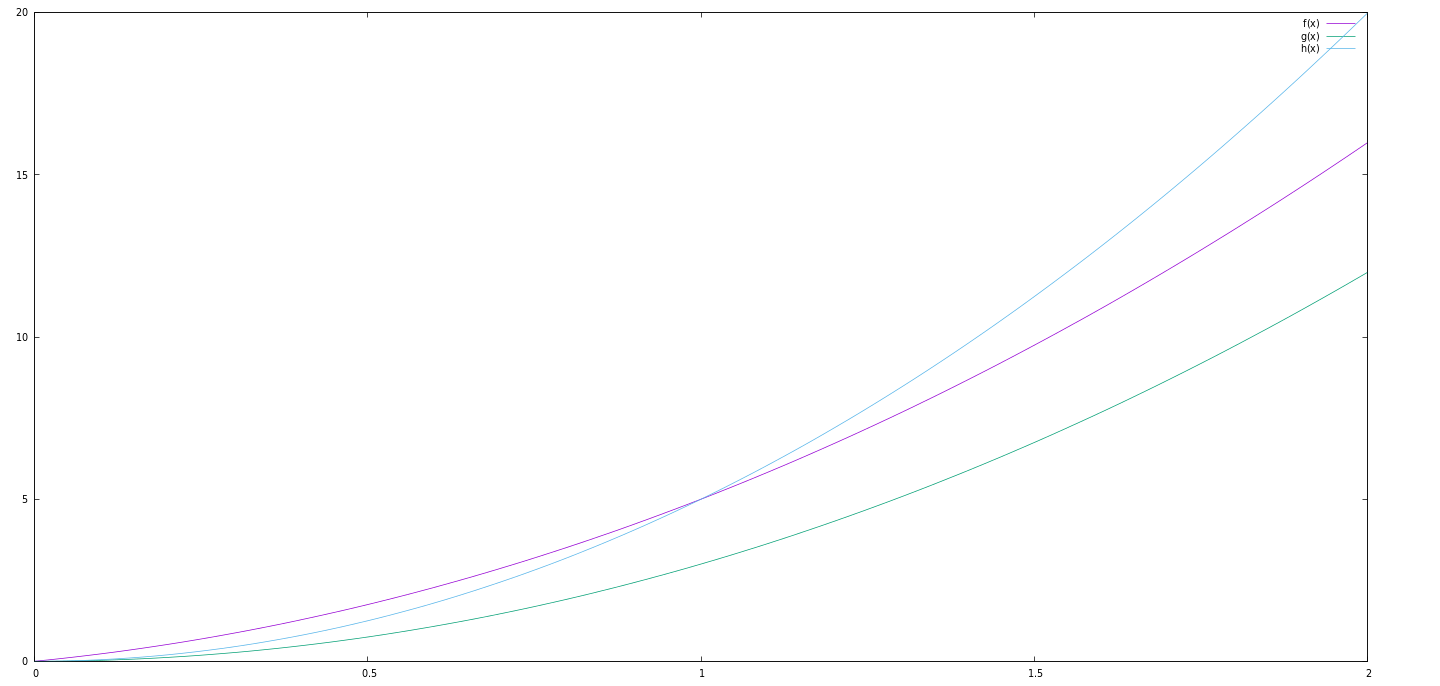
\includegraphics[width=\textwidth]{imagens/grafico5.png}
\caption{A função $f(x) = 3n^2 + 2n$ cresce de maneira assintóticamente equivalente a função $n^2$ porque $g(x) = 5n^2$ cresce mais rápido que $f$ e $h(x) = 3n^2$ cresce mais devagar que $f$.}
\end{figure}
\end{example}

\begin{example}
  \begin{displaymath}
    4  n^4 - 2 n^2 + 2 \in \Theta(n^4) 
  \end{displaymath}

   Para mostrar isso, temos que encontrar constantes $c_1$, $c_2$ e $n_0$ tais que $0 \leq c_1 n^4 \leq 4 n^4 + 2 n^2 + 2 \leq c_2 n^4$ para todo $n \geq n_0$.

   Novamente, para $n \geq 1$, $n^4$ é sempre positivo e podemos dividir tudo por $n^2$ para obter:

  \begin{displaymath}
   c_1 \leq 4 - \frac{2}{n^2} + \frac{2}{n^4} \leq c_2
  \end{displaymath}

  O valor da função $4  \frac{2}{n^2} + \frac{2}{n^4}$ é maior do que $2$ para e menor do que $6$ qualquer valor $n \geq 1$.

  Assim, temos que para todo $n \geq 1$:

  \begin{displaymath}
   2n^4 \leq 4n^4 -2n^2  + 2 \leq 6n^4
  \end{displaymath}

  \begin{figure}
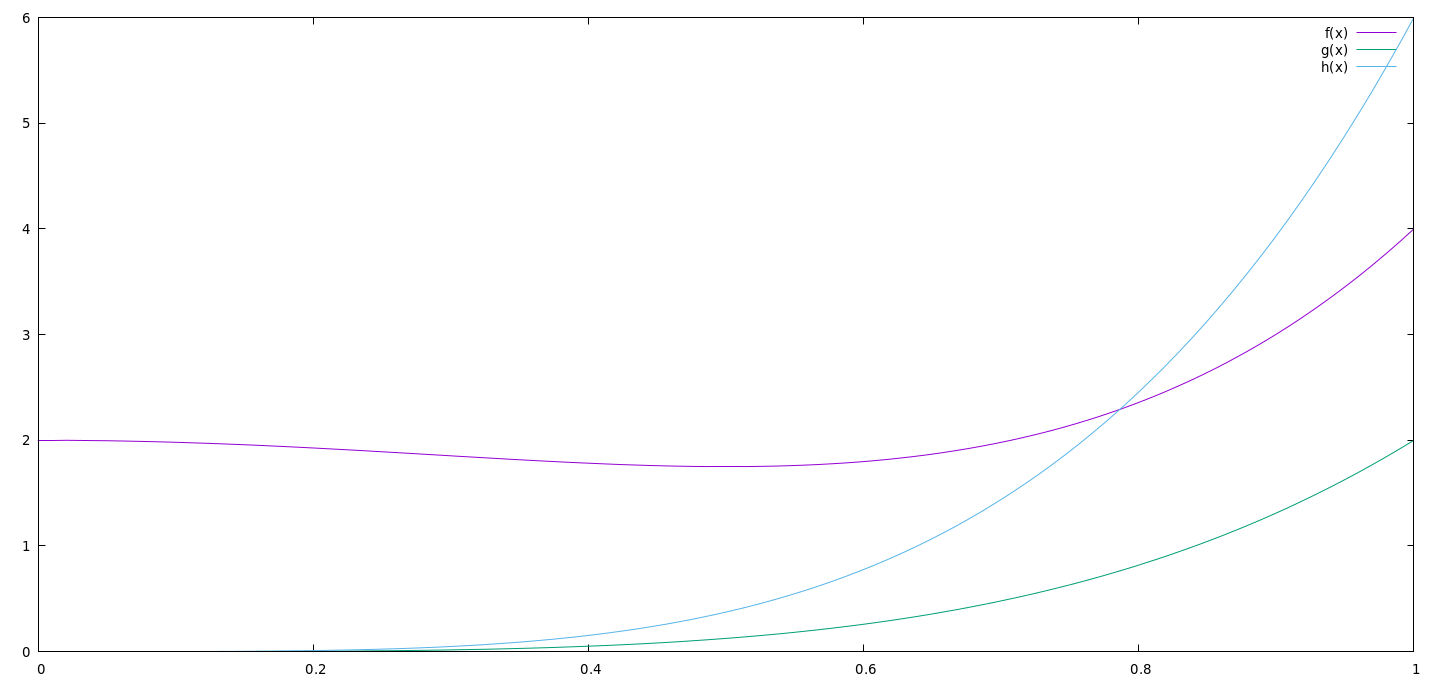
\includegraphics[width=\textwidth]{imagens/grafico6.png}
\caption{A função $f(x) = 2n^4 - 2n + 2$ cresce de maneira assintóticamente equivalente a função $n^4$ porque $g(x) = 6n^4$ cresce mais rápido que $f$ e $h(x) = 2n^4$ cresce mais devagar que $f$.}
\end{figure}

  
\end{example}

\begin{example}
  \begin{displaymath}
  2n^3 \notin \Theta(n^2)
  \end{displaymath}

  Suponha por absurdo que existam $c$, e $n_0$ tais que $2n^3 \leq c$ para todo $n \geq n_0$.

  Considerando $n > 0$ e dividindo os dois lados por $n^2$, temos:
  \begin{displaymath}
    2n \leq c
  \end{displaymath}

  Mas não é difícil ver que $2n > c$ assim que $n \geq \frac{c}{2}$, contrariando a suposição.
\end{example}

Os últimos três exemplos sugerem uma regra geral: todo polinômio é assintoticamente equivalente ao seu fator dominante.

De fato, esse resultado pode ser enunciado formalmente:

\begin{theorem}
  Seja $p(n) = a_dn^d + a_{d-1}n^{d-1} + \dots + a_0$ com $a_d > 0$ então $p(n) \in \Theta(n^d)$
\end{theorem}

\begin{corollary}
  \begin{displaymath}
    a \cdot n + b \in \Theta(n)
  \end{displaymath}
\end{corollary}

Dizemos que o consumode de tempo do algortimos Busca Sequencial é $\Theta(n)$, ou simplesmente que o algoritmo é {\em linear}.

Já o consumo de tempo do algoritmo Busca Binária, como mostra o próximo exemplo, é $\Theta(log(n))$, ou {\em logarítmico}.

\begin{example}
  \begin{displaymath}
    a \cdot log_2(n) + b \in \Theta(log(n)) 
  \end{displaymath}

   Para mostrar isso, temos que encontrar constantes $c_1$, $c_2$ e $n_0$ tais que $0 \leq c_1 log(n) \leq a \cdot log_2(n) + b \leq c_2 log(n)$ para todo $n \geq n_0$.

   Dividindo tudo por $log(n)$, temos:

   \begin{displaymath}
     c_1 \leq \frac{a}{log(2)} + \frac{b}{log(n)} \leq c_2 
   \end{displaymath}

   Fica fácil ver que as inequações valem para $c_1 = \frac{a}{log(2)}$ e $c_2 = \frac{a}{log(2)} + b$ para qualquer $n \geq 1$.   
\end{example}

Algumas classes de funções são bastante recorrentes ao analisar o tempo de processamento de algoritmos, tanto que nos referiremos a elas por um nome específico:

\begin{itemize}
\item Constante $\Theta(1)$
\item Linear $\Theta(n)$
\item Logarítmico $\Theta(log(n))$
\item Linearítmico $\Theta(n.log(n))$
\item Quadrático $\Theta(n^2)$
\item Cúbica $\Theta(n^3)$
\item Exponencial $\Theta(2^n)$
\end{itemize}

Embora a notação $\Theta$ represente um conjunto de funções, abusaremos um pouco dela para usá-la em equações.
Assim, quando escrevermos por exemplo $n\Theta(n) = \Theta(n^2)$ o que queremos dizer é que para qualquer $f(n) \in \Theta(n)$ temos que $n.f(n) \in \Theta(n^2)$.
De fato, podemos mostrar isso:

\begin{example}
  \begin{displaymath}
    n\Theta(n) = \Theta(n^2)
  \end{displaymath}

  Se $f(n) \in \Theta(n)$ então, por definição, existem $c_1$, $c_2$ e $n_0$ tais que:
  \begin{displaymath}
    0 \leq c_1 \cdot n \leq f(n) \leq c_2 \cdot n \textrm{ para todo } n \geq n_0
  \end{displaymath}
  Considerando $n_0 > 0$ e multiplicando tudo por $n$ temos que:
    \begin{displaymath}
    0 \leq c_1 \cdot n^2 \leq n \cdot f(n) \leq c_2 \cdot n^2 \textrm{ para todo } n \geq n_0
  \end{displaymath}
\end{example}

Considere mais uma vez o algoritmo da Busca Sequencial.
As duas primeiras linhas são executadas $\Theta(n)$ vezes no pior caso.
Já as duas últimas $\Theta(1)$ vezes.

Como isso temos que o tempo de execução em função do tamanho da entrada $n$ no pior caso segue a seguinte função:

\begin{displaymath}
  T(n) = \Theta(n) + \Theta(n) + \Theta(1) = \Theta(n)
\end{displaymath}

\begin{example}

  Primeiro note que $\Theta(1)$ é uma constante.
  Isso porque, por definição temos que:

  \begin{displaymath}
    0 \leq c_1 \leq f_3(n) \leq c_2 \textrm{ para todo } n \geq n_1
  \end{displaymath}

  As outras duas funções precisam respeitar as seguintes inequações:

  \begin{displaymath}
    0 \leq c_3\cdot n \leq f_1(n) \leq c_4 \cdot n\textrm{ para todo } n \geq n_2
  \end{displaymath}

  \begin{displaymath}
    0 \leq c_5 \cdot n \leq f_2(n) \leq c_6 \cdot n\textrm{ para todo } n \geq n_3
  \end{displaymath}

  Somando $f_1$ e $f_2$ temos que:

  \begin{displaymath}
    0 \leq (c_3 + c_5)n \leq f_1(n) + f_2(n) \leq (c_4 + c_6)n\ \forall n \geq max(n_1,n_2)
  \end{displaymath}
  
  Se somarmos $f_3$, certamente não alteramos as inequações do lado esquerdo e do lado direito temos:

  \begin{displaymath}
    f_1(n) + f_2(n) + f_3(n)\leq (c_2 + c_4 + c_6)n\ \forall n \geq max(n_1,n_2,n_3,1)
  \end{displaymath}
  
\end{example}

  A notação $\Theta$ indica limites inferior e superior para o crescimento de uma função.
  Quando avaliamos o tempo e processamento de um algoritmo, é comum desejarmos garantir que ele seja suficientemente eficiente.
  Ou seja, em geral queremos estabelecer apenas o {\em limite assintótico superior}.
  Para tanto, utilizamos a notação $O$.

  \begin{displaymath}
    O(g(n) := \{f(n) : \exists c, n_o \textrm{ tais que } 0 \leq f(n) \leq cg(n)\ \forall n \geq n_0 \}
  \end{displaymath}

  Sempre que $f(n) \in \Theta(g(n))$ temos que $f(n) \in O(g(n))$.
  Ou seja, $\Theta(g(n)) \subseteq O(g(n))$.
  Já a recíproca não é necessariamente verdadeira:

  \begin{example}
    $n \notin \Theta(n^2)$, mas $n \in O(n^2)$

    A primeira parte é totalmente análoga ao Exemplo \ref{}.
    Para mostrar a segunda, note que:

    \begin{displaymath}
     0 \leq n \leq n^2 \textrm{ para todo } n \geq 1
    \end{displaymath}
  \end{example}

  Da mesma forma, existem situações em que nos interessa apenas o {\em limite assintótico inferior} de uma função.
  Por exemplo, quando avaliamos certos problemas computacionais, em alguns casos específicos sabemos que é impossível resolver o problema de maneira assintoticamente mais eficiente do que certa função $f(n)$.
  Nesses casos, dizemos que o problema é $\Omega(f(n))$.

  \begin{displaymath}
    \Omega(g(n) := \{f(n) : \exists c, n_o \textrm{ tais que } 0 \leq cg(n) \leq f(n)\ \forall n \geq n_0 \}
  \end{displaymath}

  Quando temos uma solução $O(g(n))$ para um problema $\Omega(g(n))$ dizemos que essa solução é {\em ótima}. 

  \begin{example}
    O problema da busca em uma sequência arbitrária é $\Omega(n)$.
    Isso porque precisamos consultar todos $n$ elementos da sequência para saber se o elemento pertence a ela ou não.

    Assim, o algoritmo de BuscaSequencial que temos estudado é ótimo para o problema da busca em sequência arbitrária, mas ele não é ótimo para o problema da busca em sequência ordenada.
    Para este segundo problema conhecemos uma solução $O(log(n))$.
  \end{example}

  \begin{theorem}
    Para qualquer função $g(n)$ temos que $f(n) \in \Theta(g(n))$ se e somente se $f(n) \in O(g(n))$ e $f(n) \in \Omega(g(n))$. Em outras palavras: $\Theta(g(n)) = O(g(n)) \cap \Omega(g(n))$
  \end{theorem}

  Quando analisamos o tempo de processamento de um algoritmo como uma função do tamanho da entrada, é consensual a simplificação de desprezar os termos não dominantes e, com isso, simplificar as contas considerando apenas o comportamento assintótico.
  Há uma controvérsia, porém, sobre a constante multiplicadora do fator dominante.
  Alguns autores a desprezam por se tratar de um valor que depende do contexto.
  Outros autores, avaliam que esse valor não deve ser desprezado.
  No primeiro caso, utilizamos a notação $\Theta$ já apresentada.
  No segundo caso, utilizamos a notação til ($\sim$).

  Assim, por exemplo, temos que:

  \begin{displaymath}
    4n^3 + 2n + 8 \sim 4n^3 \in \Theta(n^3)
  \end{displaymath}

  Já um exemplo negativo seria:

  \begin{displaymath}
    4n^3 + 2n + 8 \nsim 2n^3 
  \end{displaymath}

  Formalmente, dizemos que $f(n) \sim g(n)$ se e somente se $lim_{n \to \infty}\frac{f(n)}{g(n)} = 1$.
  
  
\begin{exercicio}
  Mostre que o tempo de processamento do algorítimo $3Soma$ é $\Theta(n^3)$ no pior caso.
\end{exercicio}

\chapter{Algoritmos de Ordenação}

O problema da ordenação é central na análise de algoritmos por dois motivos.
Em primeiro lugar, ele é um problema com muitas aplicações em diversas áreas da computação.
Em segundo lugar, são conhecidas diversas soluções bem diferentes para esse problema, o que o torna um excelente exemplo para a teoria que estamos apresentando.

Vamos relembrar o problema:
\vspace{1em}

  {\bf Problema da ordenação}\\

  {\bf Entrada:} Uma sequência de $n$ valores $a_1, \dots, a_n$ em que $a_i \in \mathbb{Z}$ para $1 \leq i \leq n$.\\

  {\bf Saída:} Uma permutação da sequência de entrada $a'_1, \dots, a'_n$ tal que $a_i \leq a_j$ para todo $i < j$.

  \section{Selection Sort}

  Comecemos com uma solução bem simples para o problema, um algoritmo chamado Selection Sort.
  Esse algortimo consiste em identificar o maior elemento da sequência e trocá-lo com o último e repetir o processo até que todos estejam em ordem.

  Assim, podemos começar com a seguinte sub-rotina:

  \begin{codebox}
    \Procname{$\proc{Maximo}(A)$}
    \li \Comment Recebe uma sequência $a_1, \dots, a_n$
    \li \Comment Devolve $i$ tal que $a_i$ é o maior elemento da sequência
    \li $imax \gets 0$
    \li \For $i \gets 2$ até $n$
    \li \Do \If $a_i > a_{imax}$
    \li     \Then $imax \gets i$
        \End
    \End
    \li \Return $imax$
  \end{codebox}

  Para provar que este algoritmo é correto, note que a seguinte propriedade é invariante na linha 2:

  \begin{center}
    $a_{imax}$ é o maior elemento em $a_i, \dots, a_{i-1}$ 
  \end{center}

  {\em Inicialização:} na primeira vez que passamos pela linha 2 temos que $i = 2$.
  Portanto, a sequência $a_1, \dots, a_{i-1}$ tem apenas um elemento ($a_1$) que só pode ser o maior.

  {\em Manutenção:} se na iteração anterior $a_{imax}$ era o maior elemento em $a_1, \dots, a_{i-1}$ temos duas possibilidades: se $a_i$ fosse maior que $a_{imax}$ então teríamos atualizado $imax$ e ele continuaria sendo o maior da sequência, caso contrário $imax$ não teria sido atualizado, mas $a_{imax}$ continuaria sendo o maior elemento.

  {\em Término:} quando chegamos na linha 5 temos que $a_{imax}$ é o maior elemento de $a_1, \dots, a_n$.

  \vspace{1em}

  Analisar o tempo de processamento deste algoritmo também é simples.
  Para facilitar as contas, faremos mais uma simplificação.
  Ao invés de somar o tempo de processamento de cada linha, calcularemos o tempo apenas de uma das linhas que mais se repete, neste caso escolhemos a 3.
  Essa linha é processada $n$ vezes e, portanto, o algortimo é $\Theta(n)$.

  Apresentemos agora o algoritmo Selection Sort.

  
  \begin{codebox}
    \Procname{$\proc{SelectionSort}(A)$}
    \li \For $j \gets n$ até $2$
    \li \Do $imax \gets Maximo(a[1:j])$
    \li     \Then $a_{imax} \leftrightarrow a_j$
        \End
  \end{codebox}

  A propriedade invariante depois da linha 3, neste caso, é:
  \begin{center}
    $a_j, \dots, a_n$ está em ordenada e $a_j$ é o maior elemento de $a_1, \dots, a_j$
  \end{center}

  {\em Inicialização:} Na primeira passagem temos que $j=n$ e, portanto a squência $a_j, \dots, a_n$ tem um único elemento $a_n$, além disso, pela correção do algoritmo $Maximo$, $a_n$ é o maior elemento da sequência $a_1, \dots, a_n$.

  {\em Manutenção:} Pela hipótese de indução $a_j, \dots, a_n$ estava ordenada na iteração anterior e $a_j$ é o maior elemento de $a_1, \dots, a_j$, assim $a_{j-1} \leq a_j$ e temos que $a_{j-1}, \dots, a_n$ está em ordem crescente.
  Além disso, pela correção do algortimo $Maximo$ temos que $a_{j-1}$ é o maior elemento em $a_1, \dots, a_{j-1}$.

  {\em Término:} Quando saimos do laço, $j=2$ e o invariante garante, portanto, que $a_2, \dots, a_n$ está ordenado.
  Além disso, ele garante que $a_2$ é o maior elemento da sequência $a_1, a_2$.
  Concluímos que ao término $a_1, \dots, a_n$ está ordenado.

  \vspace{1em}
  

  Para analisar o tempo de processamento deste algoritmo, consideraremos a linha 2 que se repete $n$ vezes.
  A operação executada nessa linha, porém, não é atômica.
  Como vimos, ela toma tempo proporcional ao tamanho da entrada que varia em cada iteração.
  Na primeira iteração toma tempo proporcional a $n$, na segunda $n-1$, então $n-2$ e assim por diante.

  O tempo de processamento em função do tamanho $n$ da entrada, então, é:

  \begin{displaymath}
    T(n) = n + (n-1) + (n-2) + \dots + 1 = \sum_{i=1}^{n}i = \frac{n(n+1)}{2} \in \Theta(n^2)
  \end{displaymath}

  Assim se calcularmos o tempo de processamento de uma implementação desse algoritmo para entradas de diferentes tamanhos, devemos observar uma parábola (Figura \ref{}):

  \begin{figure}
    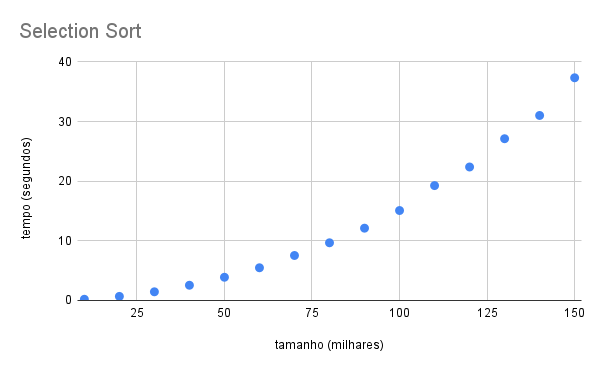
\includegraphics[width=\textwidth]{imagens/SelectionSort1.png}
  \end{figure}

  Podemos testar que se trata de fato de uma parábola poltando os mesmo valores em um gráfico em que ambos os eixos estão em escala logarítmica.
  Se a função tiver o formato $T(n) = an^2$, como nossa análise sugere, ao aplicar o $log$ nos dois lados, temos que:
  \begin{displaymath}
  log(T(n)) = log(an^2) = 2(log(n) + log(a)) = 2log(n) + 2log(a)
  \end{displaymath}
  
  Assim, o que obtemos é a equação de uma reta com inclinação $2$.
  Na Figura \ref{} observamos que de fato em uma gráfico log-log o que obtemos é uma reta com inclinação $1,94$, valor bem próximo do esperado.

  \begin{figure}
    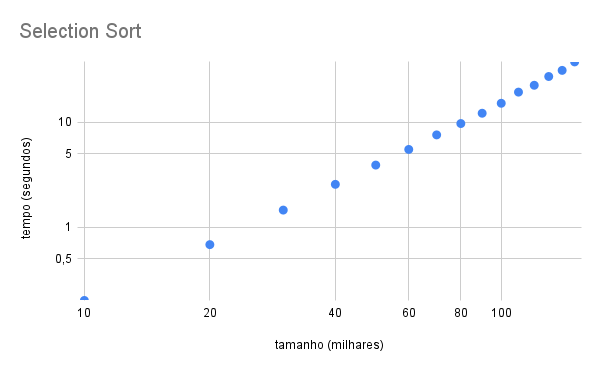
\includegraphics[width=\textwidth]{imagens/SelectionSort2.png}
  \end{figure}

  
  \section{Insertion Sort}

  Nosso segundo algoritmo segue uma ideia também simples.
  Ele ordena uma sequência de maneira análoga a forma como muitas pessoas ordenam cartas de baralhos nas mãos.

  A princípio as cartas estão todas viradas para baixo.
  Elas são inseridas uma por uma na mão do jogador cada qual em sua posição relativa correta.

   \begin{codebox}
     \Procname{$\proc{InsertionSort}(A)$}
     \li \For $j \gets 2$ até $n$
     \li $chave \gets a_j$
     \li    \For $i \gets j-1$ até $1$
     \li    \Do $a_{i+1} \gets a_i$
     \li       \If $a_i > chave$
     \li       \Then sai do laço
               \End
            \End
     \li    $a_{i+1} \gets chave$
     \End
   \end{codebox}

   Para provar a correção deste algoritmo, note que a seguinte propriedade é invariante na linha 2:

   \begin{center}
     a sequência $a_1, \dots, a_{j-1}$ está em ordem crescente
   \end{center}

   A análise do consumo de tempo é similar à do SelectionSort.
   Uma diferença está no fato de que independente da entrada, o SelectionSort sempre processa todos elementos já o InsertionSort pode sair do laço interno precocemente.
   Note então que, quando o pior caso ocorre quando os elementos originalmente estão em ordem descrescente.
   Neste caso, a análise do consumo de tempo é idêntica à do SelectionSort:

   \begin{displaymath}
     T(n) = n + (n-1) + (n-2) + \dots + 2 = \sum_{i=2}^n = \frac{n(n+1)}{2} - 1 \in \Theta(n^2)
   \end{displaymath}

   Assim, no pior caso os algoritmos são identícos.
   Veremos como analisar o caso médio na seção sobre o QuickSort, por ora basta dizer que ela também é $\Theta(n^2)$ neste caso, porém a constante multiplicadora é menor.
   Isso fica evidente quando verificamos o modelo.
   Plotando o tempo e processamento dos dois algoritmos que vimos até aqui em um mesmo gráfico com escala log nos dois eixos, vemos que ambos apresentamos uma reta praticamente com a mesma inclinação -- o primeiro tinha inclinação 1,94 e este 1,88.
   A diferença é no fato de deslocamento vertical que indica uma diferença no fator multiplicador do termo dominante.
   Essa diferença é significativa porque testamos o algoritmo com uma entrada aleatória e, nesse caso, o InsertionSort é um pouco mais eficiente:

   
  \begin{figure}
    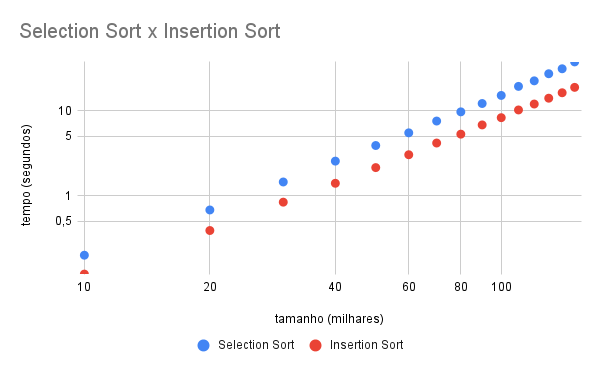
\includegraphics[width=\textwidth]{imagens/SelectionInsertion.png}
  \end{figure}   
  
\section{Merge Sort}

Antes de apresentar o próximo algoritmo, estudaremos um paradigma de projeto de algoritmos chamado {\em divisão-e-conquista} que consiste nos seguintes passos:

\begin{itemize}
  \item {\em Divisão:} a instância original do problema é dividida em um número de instâncias menores.
  \item {\em Conquista:} instâncias suficientemente pequenas são resolvidas diretamente.
    \item {\em Combinação:} se necessário, as soluções das instâncias menores são combinadas em para resolver a instância original.
\end{itemize}

Para exemplificar o paradigma, revisitaremos o algoritmo da busca binária em uma versão recursiva.

\begin{codebox}
  \li \Comment recebe uma sequência ordenada $a_1, \dots, a_n$ e um valor $b$
  \li \Comment devolve V se $b$ está na sequência e F c.c.
  \Procname{$\proc{BuscaBinaria}(A, b)$}
  \li \If $n = 1$
  \li \Then \If $a_1 = b$
  \li \Then \Return V
  \End
  \li \Else
  \li \Return F
  \End 
  \li $m \gets \left \lfloor{\frac{n}{2}}\right\rfloor$
  \li \If $b \leq a_m$
  \li     \Then \Return $BuscaBinaria(A[1:m])$
  \End
  \li \Else \Return $BuscaBinaria(A[m+1:n])$
  \End
\end{codebox}

As linhas 1 a 5 resolvem o caso base ({\em conquista}) enquanto as linhas 6 a 10 dividem o problema em instâncias menores.
Neste caso, não há necessidade de combinar as soluções pois a cada passo, metade da instância original pode ser ignorada.

Para analisar o tempo de processamento deste algoritmo primeiro estabelecemos que as linhas 1 a 5 tomas tempo constante ($c_2$), assim comas as linhas 6, 7 e 9 ($c_1$).
Jás as linhas 8 e 10 são chamadas recursivas.
Assim, o tempo de processamento do pior caso em função do tamanho da entrada $n$ é descrito pela seguinte recorrência:

\begin{eqnarray*}
  T(n) & = & c_1 + T(\left \lceil{\frac{n}{2}}\right \rceil) \\
  T(1) & = & c_2
\end{eqnarray*}

Resolveremos essa recorrência utilizando o método da árvore de recorrência:

% Árvore de recorrência
\begin{center}
\begin{tikzpicture}
\node {$T(n)$}[sibling distance = 6cm]
child {node {$T(\frac{n}{2}) + c_1$}[sibling distance = 3cm] 
  child {node {$T(\frac{n}{4}) + c_1$}
    child {node {$T(\frac{n}{2^i}) + c_1$} edge from parent [dashed]
      child {node {$T(\frac{n}{n}) + c_1$} 
        child {node {$c_2$} edge from parent [solid]}}}}};
\end{tikzpicture}
\end{center}

A árvore chega no caso base $T(1)$ quando $2^i = n$, ou seja, quando $i = lg(n)$.
Portanto, a altura da árvore é $lg(n)$.
Em cada passo, é somado $c_1$ e no último é somado $c_2$.
Concluímos que:

\begin{displaymath}
  T(n) = c_1.lg(n) + c_2
\end{displaymath}


Talvez um exemplo melhor do paradigma da divisão-e-conquista seja um versão do algoritmo de busca para sequências arbitrárias.
Dividiremos a sequência ao meio, mas neste caso, é preciso buscar nas duas metades dela.
Por fim, precisamos combinar os resultados.
O elemento $b$ está na sequência se ele está na metade direita ou na metade esquerda.

\begin{codebox}
  \li \Comment recebe uma sequência $a_1, \dots, a_n$ e um valor $b$
  \li \Comment devolve V se $b$ está na sequência e F c.c.
  \Procname{$\proc{BuscaRecursiva}(A, b)$}
  \li \If $n = 1$
  \li \Then \If $a_1 = b$
  \li \Then \Return V
  \End
  \li \Else
  \li \Return F
  \End 
  \li $m \gets \left \lfloor{\frac{n}{2}}\right\rfloor$
  \li \Return $BuscaRecursiva(A[1:m])$ ou $BuscaRecursiva(A[m+1:n])$
  \End
\end{codebox}

Como no exemplo anterior, o caso base (linhas 3 a 7) toma tempo constante $c_2$ e as operações de divisão, atribuição e o ou lógico (linhas 8 e 9) também tomam tempo constante $c_2$.
Desta vez, porém, a recursão é aplicada nas duas metades da sequência.
Assim, a recorrência que devemos resolver é:

\begin{eqnarray*}
  T(n) & = & c_1 + T(\left \lceil{\frac{n}{2}}\right \rceil) + T(\left \lfloor{\frac{n}{2}}\right \rfloor)\\
  T(1) & = & c_2
\end{eqnarray*}

Para calcular o resultado dessa recorrência, vamos novamente analisar sua árvore:

% Árvore de recorrência
\begin{center}
\begin{tikzpicture}
\node {$T(n)$}[sibling distance = 6cm]
child {node {$T(\frac{n}{2}) + c_1$}[sibling distance = 3cm]
  child {node {$T(\frac{n}{4}) + c_1$}
    child {node {$T(\frac{n}{2^i}) + c_1$} edge from parent [dashed]
      child {node {$T(\frac{n}{n}) + c_1$} 
        child {node {$c_2$} edge from parent [solid]}}}}
  child {node {$T(\frac{n}{4}) + c_1$}
    child {node {$T(\frac{n}{2^i}) + c_1$} edge from parent [dashed]
      child {node {$T(\frac{n}{n}) + c_1$} 
        child {node {$c_2$} edge from parent [solid]}}}}}
child {node {$T(\frac{n}{2}) + c_1$}[sibling distance = 3cm] 
  child {node {$T(\frac{n}{4}) + c_1$}
    child {node {$T(\frac{n}{2^i}) + c_1$} edge from parent [dashed]
      child {node {$T(\frac{n}{n}) + c_1$} 
        child {node {$c_2$} edge from parent [solid]}}}}
  child {node {$T(\frac{n}{4}) + c_1$}
    child {node {$T(\frac{n}{2^i}) + c_1$} edge from parent [dashed]
      child {node {$T(\frac{n}{n}) + c_1$} 
        child {node {$c_2$} edge from parent [solid]}}}}};
\end{tikzpicture}
\end{center}

Como no caso anterior, essa árvore chega às folhas quando $2^i = n$, ou seja, quando $i = lg(n)$.
Portanto, a altura dela é $lg(n)$.
Em cada nível dessa árvore dobramos a quantidade de $c_1$ somadas.
Assim, no i-ésimo nível são somados $2^i$ constantes e no último são somados $2^{lg(n)} = n$ constantes.
Portanto, o resultado de nossa recorrência é:

\begin{eqnarray*}
  T(n) & = & c_1.\sum_{i=1}^{lg(n)}2^i + c_2.n\\
  & = & c_1.\frac{1 - 2^{lg(n)}}{1-2} + c_2.n \\
  & = & c_1.(n-1) + c_2.n \\
  & = & (c_1 + c_2).n - c_1 \\
  & \in & \Theta(n)
\end{eqnarray*}

O merge sort, ou algoritmo de ordenação por intercalação, também segue o paradigma da divisão-e-conquista.
A ideia é quebrar a instância original ao meio até que ela tenha apenas um elemento.
Neste caso, o caso base, não é preciso fazer nada pois qualquer sequência com um único elemento está trivialmente ordenada.
O segredo está na combinação das instâncias menores para resolver a instância original.
Para este passo, usaremos um algoritmo de intercalação.

Podemos enunciar o problema da intercalação da seguinte forma:


{\bf Problema da busca}\\

{\bf Entrada:} Duas sequências $a_1, \dots, a_n$ e $b_1, \dots, b_m$ ambas em ordem crescente.

{\bf Saída:} Uma sequência $c_1, \dots, c_{m+n}$ em ordem crescente cujos elementos são os mesmos das sequências da entrada.

Para resolver esse problema utilizamos o seguinte algoritmo:

\begin{codebox}
  \Procname{$\proc{Merge}(A, B)$}
  \li $i \gets 1$
  \li $j \gets 1$
  \li \For $k \gets 1$ até $n+m$
  \li \Do \If ($a_i \leq b_j$ e $i \leq n$) ou $j > m$
  \li \Then $c_k \gets a_i$
  \li $i \gets i + 1$
  \li \Else
  \li $c_k \gets b_j$
  \li $j \gets j + 1$
  \End
  \End
  \li \Return $C$
\end{codebox}

Com isso, podemos escrever o algoritmo de ordenação da seguinte forma:

\begin{codebox}
  \Procname{$\proc{MergeSort}(A, B)$}
  \li \If $n > 1$
  \li \Then  $m \gets \left \lfloor{\frac{n}{2}}\right\rfloor$
  \li $MergeSort(A[1:m])$
  \li $MergeSort(A[m+1:n])$
  \li $A \gets Merge(A[1:m], A[m+1:n])$
\end{codebox}

O caso base do algoritmo ocorre quando $n = 1$.
Neste caso, nada precisa ser feito e o tempo tomado é constante $c$.
Já a linha 4 toma tempo linear no tamanho da entrada $n$.
Com isso, temos que o tempo de execução do algoritmo em função de $n$ é:

\begin{eqnarray*}
  T(n) & = & c_1.n + T(\left \lfloor{\frac{n}{2}}\right\rfloor) + T(\left \lceil{\frac{n}{2}}\right\rceil)\\
  T(1) & = & c_2
\end{eqnarray*}

Analisaremos, então a seguinte árvore de recorrência:

% Árvore de recorrência
\begin{center}
\begin{tikzpicture}
\node {$T(n)$}[sibling distance = 6cm]
child {node {$T(\frac{n}{2}) + c_1.n$}[sibling distance = 3cm]
  child {node {$T(\frac{n}{4}) + c_1.\frac{n}{2}$}
    child {node {$T(\frac{n}{2^i}) + c_1.\frac{n}{2^{i-1}}$} edge from parent [dashed]
      child {node {$T(\frac{n}{n}) + c_1.2$} 
        child {node {$c_2$} edge from parent [solid]}}}}
  child {node {$T(\frac{n}{4}) + c_1.\frac{n}{2}$}
    child {node {$T(\frac{n}{2^i}) + c_1.\frac{n}{2^{i-1}}$} edge from parent [dashed]
      child {node {$T(\frac{n}{n}) + c_1.2$} 
        child {node {$c_2$} edge from parent [solid]}}}}}
child {node {$T(\frac{n}{2}) + c_1.n$}[sibling distance = 3cm] 
  child {node {$T(\frac{n}{4}) + c_1.\frac{n}{2}$}
    child {node {$T(\frac{n}{2^i}) + c_1.\frac{n}{2^{i-1}}$} edge from parent [dashed]
      child {node {$T(\frac{n}{n}) + c_1.2$} 
        child {node {$c_2$} edge from parent [solid]}}}}
  child {node {$T(\frac{n}{4}) + c_1.\frac{n}{2}$}
    child {node {$T(\frac{n}{2^i}) + c_1.\frac{n}{2^{i-1}}$} edge from parent [dashed]
      child {node {$T(\frac{n}{n}) + c_1.2$} 
        child {node {$c_2$} edge from parent [solid]}}}}};
\end{tikzpicture}
\end{center}

Em cada nível da árvore, é somado $2.c_1.n$.
Como a altura dessa árvore também é $lg(n)$ temos que:
\begin{displaymath}
  T(n) = 2.c_1.n.lg(n) + 2.n.c_2 \in \Theta(n.lg(n))
\end{displaymath}

Agora que vimos como resolver três recorrências diferentes usando o método da árvore de recorrência, apresentaremos um resultado geral para resolver recorrências:

\begin{theorem}[Mestre]
  Sejam $a \geq 1$, $b > 1$ e $T(n) = aT(\frac{n}{b}) + f(n)$, então:
  \begin{enumerate}
  \item se $f(n) \in O(n^{log_b(a - \epsilon)})$ para algum $\epsilon > 0$ então $T(n) \in \Theta(n^{log_ba})$
  \item se $f(n) \in \Theta(n^{log_ba})$ então $T(n) \in \Theta(n^{log_ba}lg(n))$
  \item se $f(n) \in O(n^{log_b(a + \epsilon)})$ para algum $\epsilon > 0$ e se $af(\frac{n}{b}) \leq cf(n)$ para algum $c < 1$ e todo $n$ suficientemente grande então $T(n) \in \Theta(f(n))$
  \end{enumerate}
\end{theorem}

\begin{example}
  Comecemos pela recorrência que acabamos de analisar
  \begin{displaymath}
    T(n) = 2T\left(\frac{n}{2}\right) + cn
  \end{displaymath}

  O primeiro passo é avaliar $n^{log_ba}$ que neste caso é $n^{log_22} = n$.
  Então temos que verificar se $f(n) = cn \in \Theta(n)$.
  Neste caso, isso vale.
  Portante se aplica o caso 2 do teorema e temos que:

  \begin{displaymath}
    T(n) \in \Theta(n^{log_22}.lg(n)) = \Theta(n.lg(n))
  \end{displaymath}
\end{example}

\begin{example}
  Considere a recorrência que obtivemos ao analisar a busca binária:
  \begin{displaymath}
    T(n) = T\left(\frac{n}{2}\right) + c
  \end{displaymath}

  O primeiro passo é avaliar $n^{log_ba}$ que neste caso é $n^{log_21} = n^0 = 1$.
  Então temos que verificar se $f(n) = c \in \Theta(1)$.
  Neste caso, isso vale.
  Portante se aplica o caso 2 do teorema e temos que:

  \begin{displaymath}
    T(n) \in \Theta(n^{log_21}.lg(n)) = \Theta(1.lg(n)) = \Theta(lg(n))
  \end{displaymath}
\end{example}


\begin{example}
  Considere agora a recorrência que obtivemos ao analisar a busca recursiva:
  \begin{displaymath}
    T(n) = 2T\left(\frac{n}{2}\right) + c
  \end{displaymath}

  Primeiro avaliamos $n^{log_22} = n$.
  Então temos que verificar se $f(n) = c \in \Theta(n)$.
  Neste caso, isso não é verdade $c$ cresce mais lentamente do que $n$.
  
  Se  $\epsilon = 1$ temos que $n^{log_2(2-1)} = n^0 = 1$ e $c \in O(1)$.
  Portanto podemos aplicar o caso 1 do teorema e temos que:

  \begin{displaymath}
    T(n) \in \Theta(n^{log_22} = \Theta(n^1) = \Theta(n)
  \end{displaymath}
\end{example}

\begin{example}
  Para terminar, considera a seguinte recorrência:
  \begin{displaymath}
    T(n) = 2T\left(\frac{n}{2}\right) + n^2
  \end{displaymath}

  Primeiro avaliamos $n^{log_22} = n$.
  Então temos que verificar se $f(n) = n^2 \in \Theta(n)$.
  Neste caso, isso não é verdade $n²$ cresce mais rapidamente do que $n$.
  
  Se $\epsilon = 2$ temos que $n^{log_2(2+2)} = n^2$ e $n^2 \in \Omega(n^2)$ e $2(\frac{n}{2})^2 = \frac{n^2}{2} \leq \frac{1}{2}.n^2$ para todo $n > 0$.  
  Portanto podemos aplicar o caso 3 do teorema e temos que:

  \begin{displaymath}
    T(n) \in \Theta(f(n)) = \Theta(n^2)
  \end{displaymath}
\end{example}



\section{Quick Sort}
\section{Heap Sort}


\printbibliography

%\bibliography{ref}
\end{document}
